% This file was created with tikzplotlib v0.10.1.
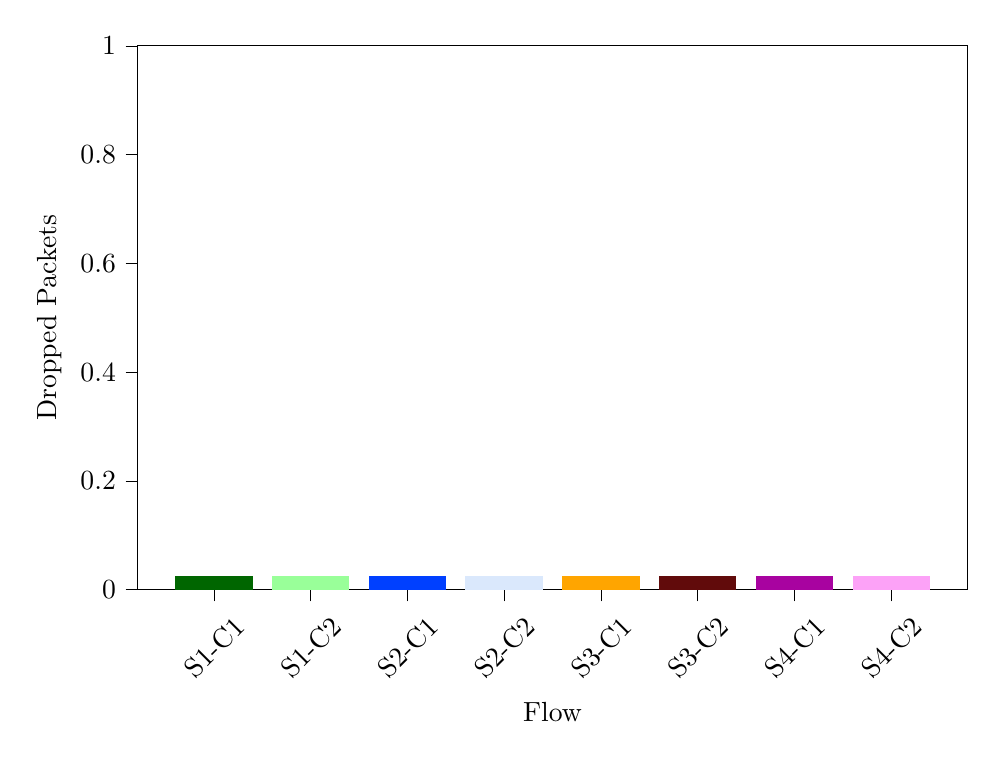
\begin{tikzpicture}

\definecolor{blue064255}{RGB}{0,64,255}
\definecolor{darkgray176}{RGB}{176,176,176}
\definecolor{darkgreen01020}{RGB}{0,102,0}
\definecolor{darkmagenta1683160}{RGB}{168,3,160}
\definecolor{lavender218232252}{RGB}{218,232,252}
\definecolor{maroon971111}{RGB}{97,11,11}
\definecolor{orange}{RGB}{255,165,0}
\definecolor{palegreen153255153}{RGB}{153,255,153}
\definecolor{violet252162247}{RGB}{252,162,247}

\begin{axis}[
height=0.7\textwidth,
tick align=outside,
tick pos=left,
width=\textwidth,
x grid style={darkgray176},
xlabel={Flow},
xmin=-0.79, xmax=7.79,
xtick style={color=black},
xtick={0,1,2,3,4,5,6,7},
xticklabel style={rotate=45.0},
xticklabels={S1-C1,S1-C2,S2-C1,S2-C2,S3-C1,S3-C2,S4-C1,S4-C2},
y grid style={darkgray176},
ylabel={Dropped Packets},
ymin=0, ymax=1,
ytick style={color=black}
]
\draw[draw=none,fill=darkgreen01020] (axis cs:-0.4,0) rectangle (axis cs:0.4,0.025);
\draw[draw=none,fill=palegreen153255153] (axis cs:0.6,0) rectangle (axis cs:1.4,0.025);
\draw[draw=none,fill=blue064255] (axis cs:1.6,0) rectangle (axis cs:2.4,0.025);
\draw[draw=none,fill=lavender218232252] (axis cs:2.6,0) rectangle (axis cs:3.4,0.025);
\draw[draw=none,fill=orange] (axis cs:3.6,0) rectangle (axis cs:4.4,0.025);
\draw[draw=none,fill=maroon971111] (axis cs:4.6,0) rectangle (axis cs:5.4,0.025);
\draw[draw=none,fill=darkmagenta1683160] (axis cs:5.6,0) rectangle (axis cs:6.4,0.025);
\draw[draw=none,fill=violet252162247] (axis cs:6.6,0) rectangle (axis cs:7.4,0.025);
\end{axis}

\end{tikzpicture}
